\BiAppChapter{外文文献译文}{}

{\noindent\textbf{题目:}破译来自9个群体的826690个个体中的骨关节炎遗传密码

\noindent \textbf{作者:}Cindy G. Boer et al.

\noindent\textbf{摘要:}}骨关节炎影响着全世界3亿多人。在此,我们对826,690名个体(177,517名骨关节炎患者)进行了全基因组关联研究荟萃分析,在11种骨关节炎表型中确定了100个独立相关的风险变异,其中52个变异先前未曾报道与骨关节炎相关。我们报告了拇指和脊柱骨关节炎的风险变异,并确定了承重和非承重关节之间的遗传效应差异。我们确定了性别特异和早期发病的骨关节炎风险位点。我们整合了来自患者原始组织(包括关节软骨、软骨下骨和骨软骨)的功能基因组学数据,并确定了高置信度的效应基因。我们提供了与疼痛(主要疾病症状)相关的表型的遗传相关性证据,并确定了与神经元过程相关的可能的致病基因。我们的结果提供了对疾病过程中的关键分子角色的诠释,并强调了有吸引力的药物靶点。我们的结果提供了对疾病过程中关键分子角色的见解,并突出了有吸引力的药物目标,以加快骨关节炎药物的转化。


\section*{绪论}

骨关节炎影响全世界超过 3 亿人。在本研究中,我们对 826,690
名个体(177,517 名患有骨关节炎)进行了全基因组关联研究Meta分析,并确定了
11 种骨关节炎表型中的 100 个独立的相关风险变异,其中 52
个以前从未被发现与该疾病相关。我们报告了拇指和脊柱骨关节炎的风险变异,并确定了负重和非负重关节之间遗传效应的差异。我们同时确定了性别特异性和早发性骨关节炎风险位点。我们整合了来自患者原发组织的功能基因组学数据(包括关节软骨,软骨下骨和骨赘软骨)并鉴定高置信度的效应基因。我们提供了与疼痛相关表型(主要疾病症状)的遗传相关性证据,并确定了与神经过程相关的可能致病基因。我们的结果提供了对疾病过程中关键分子通路的分析,并强调了可能的药物靶点。


\section*{背景}

骨关节炎是全球范围内导致残疾和疼痛的主要原因之一,有超过 3
亿人受到影响,但目前尚无治愈方法。对骨关节炎的治疗侧重于通过缓解疼痛和通过关节成形术来缓解症状。因此,我们迫切需要详细了解疾病的病因和新的药物靶点。

骨关节炎是关节的复杂退行性疾病,其特征是软骨退化、软骨下骨增厚、骨赘形成、滑膜炎症以及关节囊、韧带和相关肌肉的结构改变。近年来,全基因组关联分析
(GWAS) 在阐明骨关节炎的遗传背景方面取得了进展。迄今为止研究者们报告了 96
个统计上独立的风险变体。但这些变异只解释了一小部分表型变异且主要与影响膝关节和髋关节的骨关节炎有关。

骨关节炎会影响每个滑膜关节。研究发现体重指数(BMI)
的增加与疾病风险相关。因此我们需要需要更好地了解负重关节(膝关节、髋关节和脊柱)和非负重关节(手、手指和拇指)之间的遗传差异,以帮助解开导致疾病发展的代谢和生物机能影响。在本文中,我们对
826,690
名欧洲和东亚血统的个体的膝关节、髋关节、手指、拇指和脊柱骨关节炎表型进行了
GWAS
Meta分析。我们整合了来自疾病相关组织的功能基因组学分析,包括基因表达、蛋白质丰度和全基因组甲基化、小鼠敲除模型和单基因人类疾病表型数据,以及互补的fine-mapping、共定位和因果推理方法,以识别可能的效应基因,并通过增强我们对疾病病因学的理解促进急需的治疗转化。


\subsection*{结果}


\subsubsection*{基因结构}

\paragraph*{骨关节炎SNV的鉴定}

我们对来自 9 个人群的 13
个国际队列进行了骨关节炎的GWAS荟萃分析,涉及多达 826,690 人(177,517
名骨关节炎患者)。与迄今为止最大的骨关节炎 GWAS
相比,骨关节炎患者人数大幅增加(2.3 倍)。其中两个队列是东亚人,其中 11
个队列是欧洲血统。我们定义了 11 种表型,涵盖骨关节炎的所有主要部位(图
1;表 S1; STAR 方法)。我们使用 p \textless{} 1.3 × 10 -8的阈值发现了
11,897个全基因组显着相关的单核苷酸变异(SNV),以说明独立测试的有效数量。我们在表型中应用条件分析并确定了
223 个独立关联,其中一些在表型之间重叠。84
种变体以前与骨关节炎无关。我们调查了先前报道的骨关节炎位点,发现 96
个中的 87 个在同一方向上以名义显着性复制。

\begin{figure}[!ht]
	\centering
	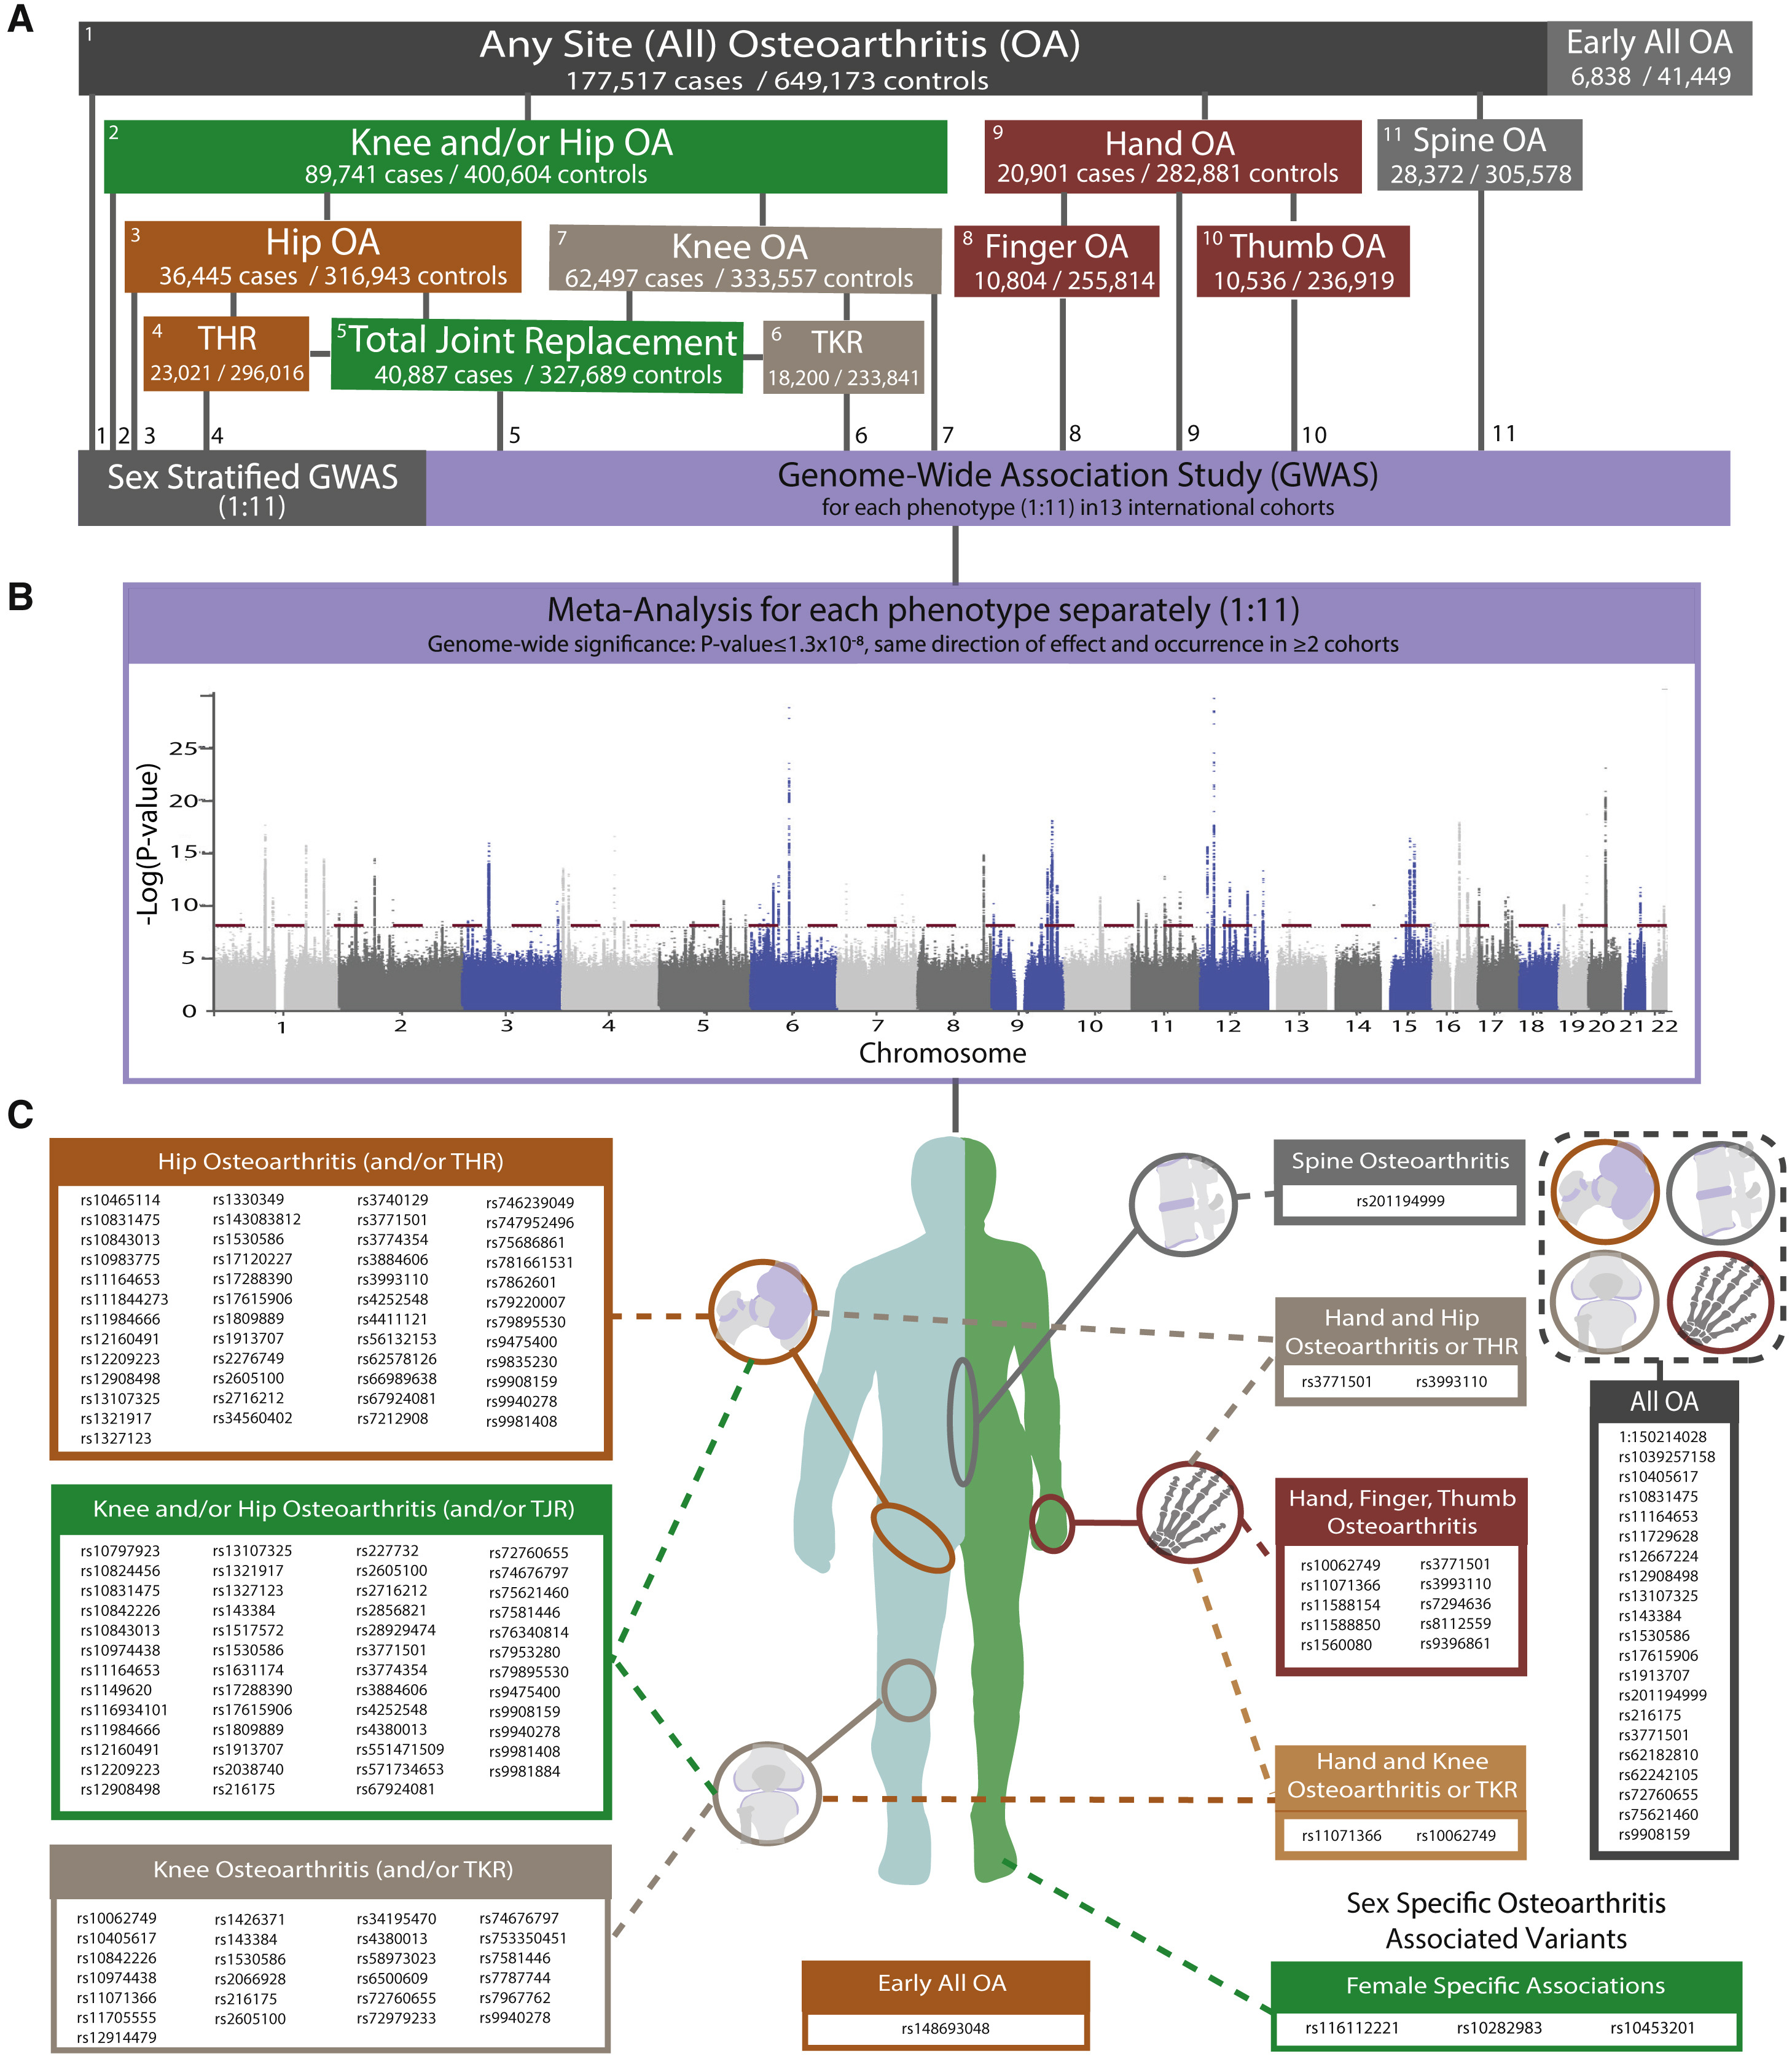
\includegraphics[width=\textwidth]{./figures/Appendix/f1.jpg}
	\caption{\textbf{基因结构} 骨关节炎的基因结构图示 A. 11种定义的骨关节炎表型的概述,特定性别分析,它们之间的关系以及它们的样本量(病例/对照)。TKR,全膝关节置换;THR,全髋关节置换。
    B. 所有11个被检查的骨关节炎表型的所有单独的元分析结果的合并曼哈顿图。虚线代表全基因组意义阈值P = 1.3 × 10-8。
    C.所有领先的全基因组意义的独立骨关节炎相关单核苷酸变异(SNVs)和与之相关的骨关节炎表型的图形概述。}
    \label{fig:app_1}
\end{figure}

我们使用条件分析来确定在疾病表型定义中不重叠的关联。我们确定了 100
个独特且独立的变异关联,其中 60
个与不止一种骨关节炎表型相关。这些变异位点中 52
个位点在先前报道中未发现与骨关节炎的关联。我们定义首要SNV
为具有最强关联统计证据的易感SNV位点。我们发现其中的六个首要SNV都在编码区(都是错义突变),59
个SNV位于基因转录本中,35 个突变发现于基因间。

本研究中,我们报告了脊柱(n = 1)和拇指(n =
2)骨关节炎的SNV位点,并增加了之前未被广泛研究就的诸如手(5 个新的,3
个先前报告的)和手指(3 个新的,2 个先前报告的)骨关节炎的风险 SNV
的数量。在 100 个 SNV 中,90 个变异基因频率较高(MAF ≥5\%),4
个变异属于低频变异( 5\%\textgreater MAF ≥0.5\%)。本研究还检测到 6
个效应量较大(OR 3.03--9.52)的罕见的变异关联 (MAF 0.03\%--0.11\%)。
除去一个已被研究发现的变异之外,其他5个变异关联是由本研究发现。而这五个新变异主要来自冰岛的一个大家系之中。

我们还对非欧洲人种0.9\%--2.8\% 的病例是东亚人种)的个体进行了关于4
种骨关节炎表型(包括脊柱、膝关节、膝关节和/或髋关节,以及任何部位的骨关节炎)的分析。尽管来自东亚人种的样本量很小,但我们观察到
62\% 的变异在东亚人群基因型信息的分析中也具有一定意义,并且这些信号中的
20\% 也具有显著的统计学意义(p = 2.27 × 10 -5)。

我们还测试了通过该变异信息构建的多基因风险评分
(PRS)模型的预测能力,我们发现处于PRS
分布的较高十分位数范围内的个体罹患骨关节炎的可能有显著升高。


\paragraph*{女性特异性骨关节炎风险变异}

为了研究仅针对男性、仅针对女性或在男性和女性中具有差异影响的骨关节炎相关变异,我们进行了性别相关关联测试以及等位基因效应的异质性测试。通过该测试我们发现了
3 个新的女性特异性SNV,其中两个显示出性别间效应大小的显著差异(Phet-diff
\textless0.016)。其中突变
rs116112221在女性的全髋关节置换表型中具有显著性,并且位于包含长基因间非编码
RNA的区域。同该区域最接近的蛋白质编码基因是\emph{FANCL} 。\emph{FANCL}
突变可能导致人类原发性卵巢功能不全,这种疾病同时会导致更年期提前,而虽然还没有有力研究论证,更年期的提前也被认为与骨关节炎患病率增加有关。临床研究表明,选择性雌激素受体调节剂(SERMs)治疗对该类型骨关节炎的预后有着积极作用,特别是对于绝经后早期或骨质疏松性骨关节炎患者。

我们进一步确定了与全髋关节置换相关的在男性和女性之间的影响具有明显差别的突变rs10282983。rs10282983
位于 \emph{C8orf34}
的内含子中,该基因被发现与腰臀比和足跟骨矿物质密度等性状有关,而两者都是可能导致骨关节炎的因素。另一突变rs10453201位于基因\emph{UBAP2}的
5'末端,该突变与任何部位的女性骨关节炎显著相关。而基因\emph{UBAP2}与帕金森病、2
型糖尿病、BMI和人体足跟骨矿物质密度都存在相关。


\paragraph*{早发性骨关节炎}

全基因组荟萃分析也确定了具有大效应量和低等位基因频率的早期骨关节炎的新风险变异rs148693048。该变异在所有荟萃研究的来源中都被报道同骨关节炎形状存在一定的相关,但是之前并没有将其与骨关节炎相关联的研究。与退化的软骨相比,附近的两个蛋白质编码基因(
\emph{
NEFM}和\emph{DOCK5})在完整的软骨中表现出显著不同的表达水平。\emph{NEFM}(神经丝介质)与神经元结构的延展有关,并且由其指导表达的蛋白质通常用作神经元损伤的生物标志物。\emph{DOCK5}
(胞质分裂作动蛋白
5)的鸟嘌呤核苷酸交换活性已被确定为破骨细胞功能的调节剂,在骨吸收中发挥重要作用,对其活性的药理抑制可防止骨质溶解,同时保持人类和小鼠的骨形成速度。\emph{DOCK5}的其他内含子变异也显示出与其他骨表型的关联(p
\textless{} 5.0 × 10 -8),例如足跟骨矿物质密度和青少年特发性脊柱侧凸。

\subsubsection*{交叉表型分析}

\paragraph*{不同表型信号的异同}

\begin{figure}[!ht]
	\centering
	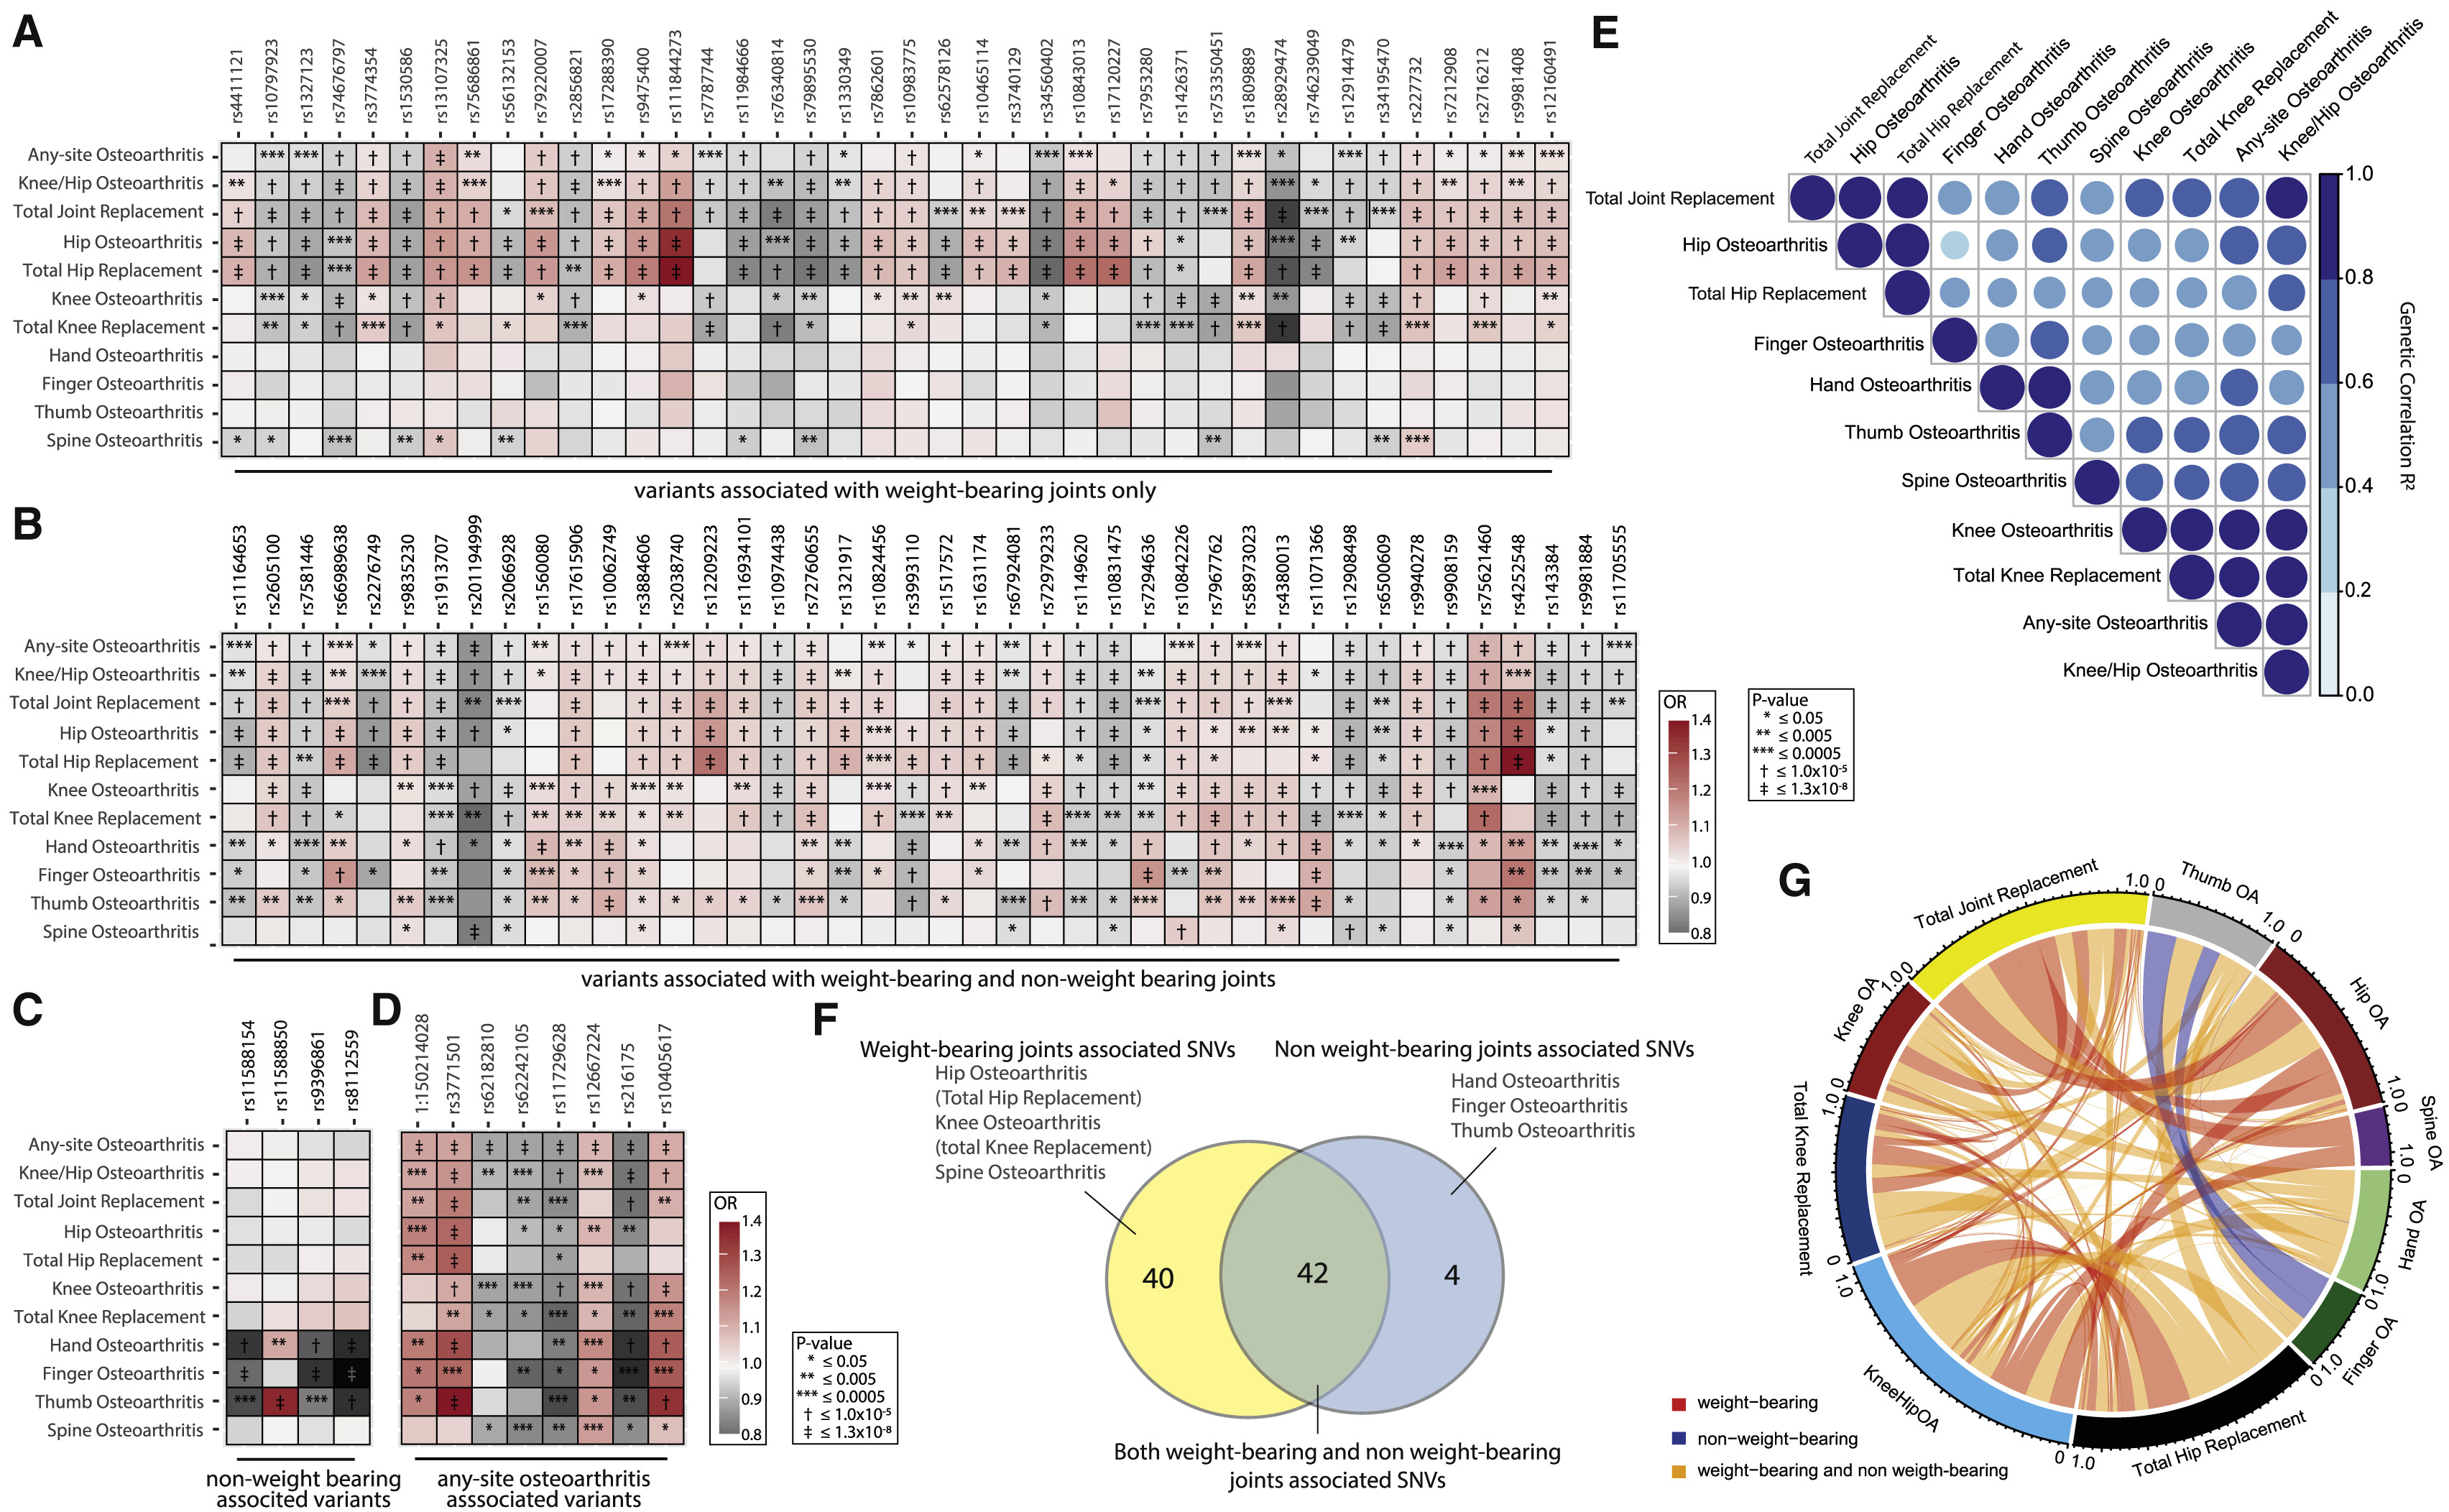
\includegraphics[width=\textwidth]{./figures/Appendix/2.jpg}
	\caption{\textbf{不同表型的信号的相似性和差异性} 骨关节炎遗传学之间的相关性和重叠性
    A-D.骨关节炎相关单核苷酸变异SNV的热图。每个骨关节炎表型GWAS结果的效果大小(OR,几率)和P值都显示在每个主导SNV上。OR以颜色表示,P值以方框内的符号表示。A.只有负重关节(髋关节、膝关节和脊柱)。B. 承重和非承重关节(髋关节、膝关节、脊柱、手、手指和拇指)。C. 非负重关节(手、手指和拇指)。D. 任何部位的骨关节炎SNVs。
    E.受检的骨关节炎表型之间的遗传相关性(R2)的热图。
    F.维恩图描述了与负重和非负重关节相关的SNVs的数量和重叠。
    (G) Circos图描述了100个主导变异的骨关节炎关联的重叠情况。}
    \label{fig:app_2}
\end{figure}

我们观察到一些变异表现出关节特异性效应。我们发现其中的60个SNV在全基因组范围内与一种以上的骨关节炎表型显著相关。其中40个SNV
仅与负重关节骨关节炎存在着全基因组上的显著关联,4 个 SNV
仅与非负重关节骨关节炎存在显著关联。我们有超过 80\%
的把握提取负重关节分析中的所有 4
种非负重特异性变异(全基因组显著性)。此外,在非负重关节(手骨关节炎)分析中,我们有超过
80\% 的把握来检测 40 个负重关节特异性效应中的 22
个。尽管已知有几种核心途径支持骨关节炎病理学,但无论受影响的关节部位如何,除了\emph{GDF5}基因座外,之前没有发现常见的遗传性骨关节炎
SNV。而在本研究中我们已经确定了 42
个在承重和非承重关节中都有很强的关联性的SNV。其中几个 SNV,包括rs3771501
( \emph{TGFA} )、rs3993110
(\emph{TEAD1/DKK3})、rs72979233(\emph{CHRDL} 2)和
rs7967762(\emph{PFKM} / \emph{WNT10B}
)与多个骨关节炎关节部位相关。这些变异可能指示了骨关节炎病理学中常见的潜在机制。它们已被证明在转化生长因子
β (TGF-β)/骨形态发生蛋白 (BMP)
、Wnt/β-catenin信号通路中发挥作用,并且其功能相互作用可能与骨关节炎的发病机制有关
。这些信号通路可能是药物开发的主要候选者。

从骨关节炎表型之间的关联信号的比较中也可以收集到更多的信息。大多数与膝关节、髋关节和膝关节和/或髋关节骨关节炎相关的
SNV
对各自的关节置换表型具有较大的影响,但是所有这些表型的样本量都较小。这可能是由表型定义的同质性驱动的,或者可以代表生物和功能的相关性,表明这些位点可能在接受关节置换(即疼痛和炎症)中发挥了比骨关节炎病理本身更重要的作用。例如,rs76340814(\emph{
PTCH1})和rs28929474(\emph{SERPINA1}的错义变体)与全髋关节置换(THR)、全膝关节置换(TKR)和全关节置换(TJR),比与髋关节或膝关节骨性关节炎有更强的关联和更大的效应值。事实上,\emph{PTCH1}
被认为在神经系统和大脑发育中发挥作用,而\emph{SERPINA1}被认为在炎症中发挥作用。对大鼠骨关节炎模型的研究表明,用\emph{SERPINA1}
编码的α-1-反蛋白酶进行早期治疗,可以阻断中性粒细胞弹性蛋白酶的蛋白溶解活性,并使关节炎症、疼痛和隐性神经损伤得到持久改善。

\paragraph*{表型之间的遗传联系}

尽管骨关节炎的遗传特性范围较广,我们还是发现骨关节炎亚型共享大量遗传成分。

我们调查了骨关节炎的遗传成分是否与其他性状共享,发现与人体测量特征(BMI、肥胖、体重和脂肪量)、2型糖尿病、教育、抑郁症状、吸烟行为、骨矿物质密度、生殖表型和智力有明显的相关性,如以前的报道,以及几种疼痛表型。

疼痛是骨关节炎患者经历的最多的致残症状,也是患者寻求医疗支持甚至全关节置换的主要原因之一。骨关节炎导致疼痛的病因是多因素的,包括明显的软组织炎症、涉及关节痛觉感受器的疼痛通路的敏感化、中枢神经系统的痛觉处理以及骨关节炎模型中的神经病理性疼痛成分。虽然疼痛是骨关节炎的主要症状,但之前的研究中没有发现骨关节炎与疼痛发生的遗传决定因素。本研究发现骨关节炎与坐骨神经痛、纤维肌痛、头痛和其他背痛表型之间有很高的相关性,其中与脊柱骨关节炎的相关性最高(遗传相关性{[}rg{]}
=
0.61、0.87、0.39和0.79)。\emph{SOX5}是本文所新发现的疼痛信号之一,之前有报道称其在人类骨关节炎软骨中的表达被上调,并与背痛和腰椎间盘退化有关。这些发现得到了动物模型数据的支持,对小鼠的研究表明\emph{SOX5}
的失活导致小鼠包括软骨、脊索或椎间盘等骨骼发育的缺陷。我们还在LD-Hub数据库中观察到骨关节炎与背痛、走路时腿痛、膝痛、髋痛、背痛和颈/肩痛等一系列疼痛表型之间有很强的相关性(均来自UKB)。因此,我们的数据表明,一部分已识别的骨关节炎相关信号也与骨关节炎疼痛有关。

\subsubsection*{效应基因和生物学途径}

\paragraph*{鉴定推定的因果变异}
我们采用了互补计算方法,将GWAS信号细化到一小部分可能的因果突变上,根据信号的富集程度确定相关的组织,并根据表达定量性状位点(eQTL)的共定位和因果推断分析提供骨关节炎致病机理上的解释。12个信号被精细地映射到完全包含在单个基因的转录本内的突变组,其后验概率大于95\%,但我们注意到这并没有为该基因为导致骨关节炎的效应基因这一推论提供结论性的证据。值但得注意的是,目前是其他适应症使用的批准药物的靶点\emph{
ALDH1A2}以99\%的后验概率精细映射到6个内含变异,这也为为药物重利用提供了潜在的机会。对于其中6
个 SNV(3 个新的和 3 个已知的),单个突变可以被假定为具有
\textgreater95\% 后验概率的因果关系。

\paragraph*{收集证据以识别效应基因}

\begin{figure}[!htbp]
	\centering
	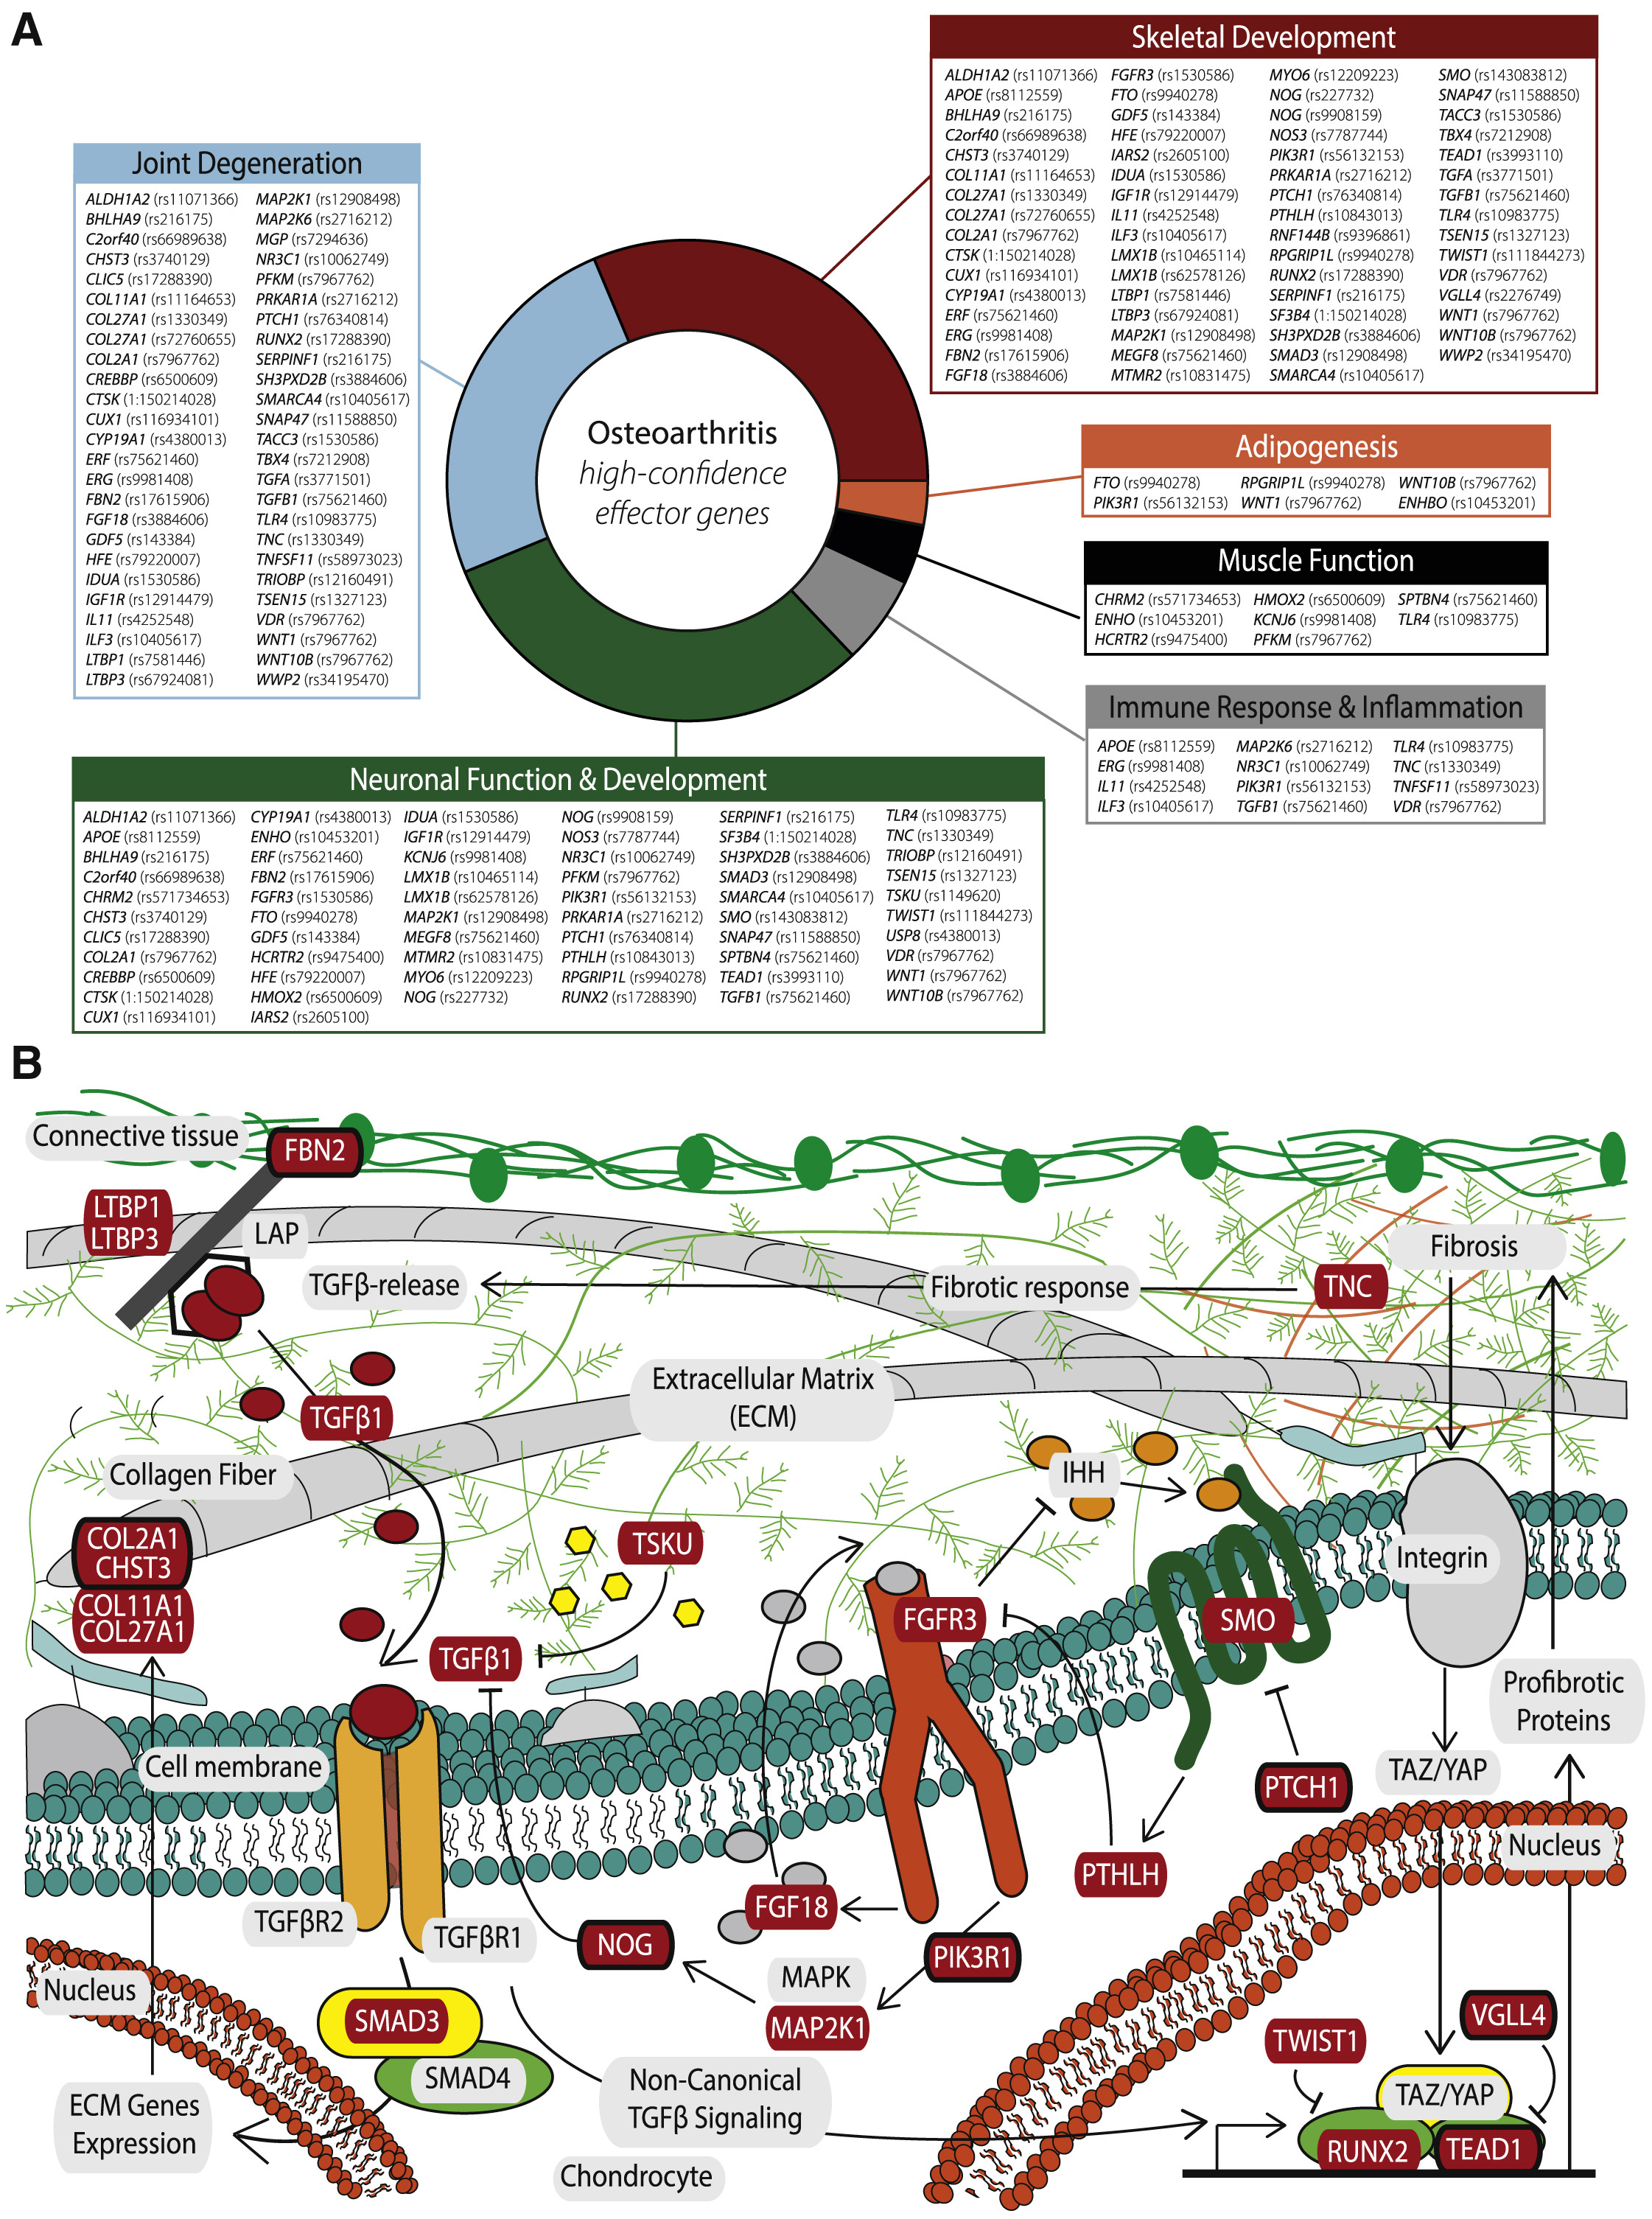
\includegraphics[width=\textwidth]{./figures/Appendix/3.jpg}
	\caption{\textbf{高置信度骨关节炎效应基因} A.77个高置信度骨关节炎效应基因及其广泛的生物分类概述,如表3和S12所描述。每个基因的主要SNV在括号中给出。
    B.软骨细胞及其细胞外基质的示意图,突出了示范性的骨关节炎相关生物途径(TGF-β信号传导,FGFR3信号传导,以及部分纤维化途径)和高置信度的效应基因(红框内),包括已确定的和新确定的(红框内有黑色轮廓),已发现其发挥的作用。
    }
    \label{fig:app_3}
\end{figure}
我们评估了在从接受关节置换手术的骨关节炎患者中提取的软骨细胞中,是否有位于骨关节炎相关变异1Mb距离内的基因在原发性骨关节炎影响的组织中表现出不同的基因表达和蛋白丰度。同样,我们比较了完整的和退化的软骨组织下的软骨下组织的基因表达。通过结合互补的功能基因组学和计算方法的结果,我们确定了637个至少有一条证据指向一个推定的效应基因的基于基因。对于这637个基因,我们结合了来自精细图谱、eQTL共定位分析、动物模型数据、人类肌肉骨骼和神经元表型数据、功能基因组学和因果推理分析等支持性信息,确定了77个至少有3条不同证据支持其作为效应基因的基因。在这77个基因中,有4个是由错义线索变异支持的(\emph{
VGLL4}中的rs2276749,\emph{CHST3}中的rs3740129,\emph{SMO}中的rs143083812,和\emph{IL11}的rs4252548);48个为以前报道的骨关节炎相关SNVs的可能效应基因提供了强有力的额外证据;
30个位于新的相关信号中。

在这些基因中,\emph{CHST3}、\emph{SMAD3}和\emph{GDF5}具有较高效应基因可信度,各有6条不同的证据支持它们同骨关节炎发展过程相关。\emph{CHST3}(碳水化合物硫酸盐转移酶3)是一个新发现的信号,它编码软骨中的主要蛋白多糖,即硫酸软骨素。\emph{
CHST3}的突变在之前的研究中被发现与身材矮小、先天性关节脱位、足癣、Larsen综合征和肘关节发育不良等性状有关。\emph{CHST3}同时也被证明与腰椎间盘退化有关。

为了进一步了解高置信度效应基因在疾病过程中的生物学作用,我们整合了基于内涵型分析的与基础生物学更密切相关单基因和罕见人类疾病数据、全表型分析和额外的功能基因组学数据等额外信息。通过综合所有的证据,我们发现77个高置信度效应基因中的几个基因被分配到穿越了多个生物学过程的可能机制中,并通过这些机制发挥其作用。我们主要关注本工作中新报道的相关基因。这些基因也是进一步机制探索和临床研究的高价值候选基因。

大多数高置信度的效应基因与骨骼发育(共63个,21个与新报告的信号相关的基因)和关节退化(共50个,18个与新报告的信号相关的基因;13个基因在骨骼发育和关节退化类别中是共同的)有关。三个由新的遗传信号产生的效应基因,即\emph{CHST3}、\emph{
COL2A1}和\emph{FBN2},编码着结构蛋白。II型胶原蛋白α1链(\emph{COL2A1})编码的是软骨的基本结构成分,对关节的形成和骨骼的生长很重要。目前已发现许多疾病都同\emph{COL2A1}
有关,包括软骨异常和骨的异常,如脊柱骨骺线发育不良、Kniest发育不良和早发性骨关节炎。纤维蛋白2(\emph{FBN2}
)编码一种在细胞外基质中形成微纤维的糖蛋白,在个体的早期形态发生过程中具有重要作用。纤维蛋白能够有效地调节免疫反应、炎症和组织平衡,在骨重塑中很重要,并且可以调节BMP和TGF-β的局部可用性。\emph{FBN2}的突变会导致契约性蛛网膜病)。

同时有几个基因与信号传导途径有关。退化样家族成员4(\emph{VGLL4})通过与TEA域(TEAD)转录因子相互作用而发挥作用。值得注意的是,我们发现另一个新的与关节置换和手部骨关节炎相关的信号位于这样的转录因子中,即\emph{TEAD1}
基因,表明这两个信号背后有一个共同的分子途径。\emph{TEAD1}在Hippo信号通路中发挥作用,并受参与机械感应和机械传导的\emph{YAP1}和\emph{TAZ}原基因蛋白的转录调控,而关节软骨的机械适应是骨关节炎的一个重要因素。同时有研究发现\emph{VGLL4}
的下调与Wnt/β-catenin通路靶基因的上调有关。

Wnt家族成员1(\emph{WNT1})和wnt家族成员10B(\emph{WNT10B})参与Wnt信号通路,在骨关节炎发病机制中具有既定作用。WNT10B的突变与肢体缺陷和牙齿异常有关,\emph{WNT1}
的突变与成骨不全症有关。胰岛素样生长因子1受体(IGF1R)具有酪氨酸激酶活性,介导胰岛素样生长因子的作用,并调节软骨矿化。

一氧化氮合酶3基因(\emph{NOS3})编码一氧化氮合酶(eNOS)的血管内皮异构体。\emph{NOS3}与小鼠的散发性肢体缺陷有关。LIM
Homeobox转录因子1β(\emph{LMX1B}
)是一种转录因子。LMX1B的突变导致一种罕见的常染色体显性疾病,其特征是指甲萎缩、髌骨发育不良或缺失,以及肘部和髂角发育不良。

Patched
1(\emph{PTCH1})编码Hh配体的受体,并调节平滑肌、毛细血管类受体(\emph{SMO}
,另一个与已知主导SNV有关的效应基因)的活性。当结合时,PTCH1放弃其对SMO的抑制作用,并激活Hh信号级联,这在控制软骨细胞的增殖中发挥了重要作用,也在软骨内层骨形成和纵向生长过程中刺激成骨作用。

还有几个新发现的高置信度效应基因与神经元有关。由\emph{C2orf40}(也叫\emph{ECRG4})编码的蛋白Augurin参与了动物模型的中枢神经系统发育,并与人类阿尔茨海默病和相关痴呆症的神经病理学特征有关。\emph{TSEN15}
附近的SNVs与骨关节炎关联的人体测量特征有很强的相关性,如身高、体脂分布和根据BMI调整的腰围。CUT样同源蛋白1(\emph{CUX1}
)是参与大脑神经元分化和突触发生的转录因子。在肢体发育过程中被观察到的Cux1在软骨间的表达,也其表明在关节形成中也有调节作用。

TRIO和f-actin结合蛋白(\emph{TRIOBP})基因通过2个启动子编码多种蛋白异构体。TRIOBP-1与TRIO和f-actin结合蛋白相互作用,共同在神经元形态发生中发挥关键作用并控制肌动蛋白细胞骨架组织、细胞运动和细胞生长。

肌管蛋白相关蛋白2(\emph{MTMR2})在膜靶向、囊泡转运和信号转导途径的调节中具有重要作用。\emph{MTMR2}
的突变导致4B型夏科-玛丽-托斯病,该病症状包含髓神经纤维普遍丧失,髓鞘局部折叠,神经对肌肉的神经信号传导不足,导致肌肉无力和萎缩。普遍表达的CREB结合蛋白(\emph{CREBBP}
)所编码的蛋白质在发育过程中起着关键作用,特别是与大脑大小调节、正确的神经细胞分化和神经前体细胞迁移有关,这些相关也在小鼠模型中得到了证明。

胆碱能受体毒蕈碱2(\emph{CHRM2})参与了细胞反应的调节。对大鼠组织的分析亦发现其在全脑和人类神经母细胞瘤细胞中的表达。\emph{CHRM2}的变异易导致包括阿尔茨海默病在内的各种神经精神疾病。突触体相关蛋白47(\emph{SNAP47}
)所编码的蛋白是一种可溶性N-乙基马来酰亚胺敏感融合蛋白受体(SNARE)蛋白,参与囊泡转运和膜融合。SNARE介导的融合是驱动突触传递、神经元发育和生长的一个重要机制。SNAP47在物质出细胞模式和神经元形态发生中发挥作用。

有几个效应基因有免疫或炎症作用。例如,Toll样受体(\emph{TLR4}
)编码的蛋白质在病原体识别和激活先天免疫反应中发挥着基本作用。TLR4也可被与肌肉骨骼病症有关的受损组织产生的宿主分子激活。该基因与软骨细胞、成骨细胞和滑膜细胞的基因表达一起,将TLR4与类风湿性关节炎、骨关节炎和骨质疏松症联系在一起。而因此,TLR4的调节或抑制已被建议作为这类疾病的一种治疗方法。T细胞的激活可以通过影响肿瘤坏死因子配体超家族成员11(\emph{
TNFSF11})的表达而导致破骨细胞生成和骨吸收。\emph{TNFSF11}
编码核因子卡帕-β配体的受体激活剂(也称为RANKL),这种细胞因子与类风湿性关节炎的炎症性骨重塑有关,TNFSF11水平的增加与关节炎严重程度的恶化有关,并在破骨细胞生成中具有一定作用。核受体亚家族3组C成员1(\emph{NR3C1}
)编码糖皮质激素受体(GR),在细胞质中循环,参与炎症反应。在骨关节炎中,成骨细胞和软骨细胞中的内源性糖皮质激素信号是有害的。

磷酸果糖激酶(PFKM)对肌肉功能有一定的作用。它编码一类肌肉同工酶,在糖酵解过程中催化果糖-6-磷酸的磷酸化。该基因的突变导致Tarui's病(糖原贮藏病7型),这是一种常染色体隐性代谢疾病,临床上以运动不耐受、肌肉痉挛、劳累性肌病和代偿性溶血为特征。

\subsubsection*{药物靶点识别}

我们检查了所有637个至少有一个来自精细映射和功能分析的支持证据的基因的成药性(Druggability)
。在这637个基因中,有205个存在于可药性基因组数据库中,致使数据库中具有支持证据的基因富集了1.46倍。从这些骨关节炎可药用的靶点基因中,有71个基因位于第一类,其中包括已批准(许可)的药物和临床开发中的药物的靶点。在有三个不同证据支持因果关系的77个基因中,有20个是一级候选基因(其中18个存在于DrugBank中),其中7个对应于本研究中发现的新基因信号(\emph{
CHST3}、\emph{VDR}、\emph{TNFSF11}、\emph{IGF1R}、\emph{NR3C1}、\emph{CHRM2}和\emph{NOS3})。

在第1类基因中,有10种候选药物先前已在骨关节炎的临床疗效试验或队列研究中得到研究(6个作用于新信号:\emph{PPARD}、\emph{NR3C1}、\emph{VDR}、\emph{MAPK14}、\emph{IGF1R}和\emph{CHST3})。\emph{PPARD}
拮抗剂舒林酸因其前列腺素合成酶活性而被授权作为非甾体抗炎药(NSAID)用于骨关节炎。\emph{SLC1A1}
激动剂和神经性疼痛抑制剂普瑞巴林是骨关节炎的常用药。普瑞巴林与非甾体抗炎药美洛昔康共同用于短期治疗膝关节骨性关节炎的疼痛,并且有一些支持性的临床试验数据。\emph{NR3C1}
编码糖皮质激素受体,该受体的激活具有广泛的抗炎和免疫调节作用。类似的,有几个激动剂分子获得了上市许可。其中,泼尼松龙长期以来一直被用作炎症性关节炎的疾病调节剂,在最近的心脏结果预防评估(HOPE)研究中,发现它能有效减少手部骨关节炎的疼痛和滑膜炎。Cathepsin
K(由\emph{CTSK}基因编码)是一种在破骨细胞内的胶原蛋白降解中起关键作用的酶,MIV-711是一种选择性的Cathepsin
K抑制剂,最近在一项2期临床试验中被证明能有效减少膝关节骨性关节炎患者的结构损伤。\emph{VDR}
编码维生素D受体,它的激活是钙代谢的一个主要调节器。补充维生素D对膝关节骨性关节炎的症状和结构损伤的临床试验结果不一,但可能对维生素D缺乏的患者稍有益处。\emph{EGLN2}
编码一种脯氨酸羟化酶EGL九号同源物2,其主要介导脯氨酸的羟化,从而促进胶原蛋白和蛋白多糖的合成。尽管效果不一,补充其激动剂抗坏血酸(维生素C)与观察人群中的关节健康有关。在日本ROAD人群中,HCAR2激动剂烟酸(维生素B3)的缺乏被发现与膝关节骨关节炎的进展有关。MAPK14拮抗剂PH-797804已经在一项2期临床试验中进行了研究以考察PH-797804单独或与萘普生一起对膝关节骨性关节炎受试者的疼痛缓解情况(NCT01102660),然而本文尚未在PubMed或ClinicalTrials.gov上发现任何试验结果报告。最后,碳水化合物磺化酶3激动剂沙利度胺已被证明可通过涉及血管内皮生长因子(VEGF)表达下调的机制,在小鼠内侧半月板失稳模型中减弱早期骨关节炎的发展。

另外45个一级可药用目标都有市场授权或正在进行其他适应症的临床开发。其中10个是高置信度的效应基因,16个为本文发现的新的遗传信号。这里介绍的关于它们在临床骨关节炎中作用的功能和流行病学证据为早期再利用调查提供了支持。一种抗体小分子,福斯塔马提尼,作为一种酪氨酸激酶抑制剂多次出现在候选药物中,它针对\emph{
AAK1}、\emph{EPHA5}、\emph{GAK}、\emph{GSK3A}、\emph{MAP2K1}、\emph{MAP2K6}、\emph{PAK1}和\emph{PRKCD}
,并作为一种生物性疾病修饰抗风湿药物(DMARD)获得了上市许可。JAK2抗体baricitinib和TYK2抗体tofacitinib都作为生物DMARDs上市,而MAP2K1抗体binimetinib作为生物DMARD目前处于3期临床试验。因此,这些药物中的每一种都为骨关节炎的再利用研究提供了临床机会和假定的机制。在其余的一级和二级可药用目标中,潜在的可药用分子处于较早的开发阶段,提供了可期的再利用机会。


\subsection*{讨论}

我们的研究结果产生了关于负重和非负重关节之间差异的进一步知识,并指出了任何关节的骨关节炎疾病发展的共同机制,以及关节类型骨关节炎中的特异性。事实上,骨和软骨的发展途径在负重和非负重关节的信号中被富集,确定了关节生长是任何形式的骨关节炎的共同机制。

我们同时在该疾病和其主要症状--疼痛之间建立分子联系。我们证明了骨关节炎和疼痛相关表型之间的遗传相关性,并确定了神经系统通路的信号富集。此外,几个高置信度的效应基因在神经病理学中也有作用。本研究中的大多数骨关节炎病例被定义为全关节置换和/或自我报告的骨关节炎,而这两种疾病表型都是由疼痛高度驱动的。这些基因的鉴定也可以对进一步的关节疼痛相关疾病产生影响,迄今为止,对这些疾病的认识还很有限。

大量的高置信度效应基因汇聚在在软骨细胞的平衡和骨质疏松中发挥着重要作用的软骨内径上。其中几个已被识别的基因在TGF-β信号传导和功能方面起到重要作用。新发现的纤维蛋白2(\emph{FBN2})信号与\emph{LTBP1}和\emph{LTBP3}
一起,调节活性TGFB1的可用性。TGFB1是软骨中TGFB的主要形式,其可以通过SMAD3信号激活一连串的包括我们目前研究中已经识别的的ECM-基因,如碳水化合物硫代转移酶3(\emph{CHST3})在内的下游基因,。

我们的数据为FGF信号级联(\emph{FGFR3}、\emph{FGF18}和\emph{PIK3R1})参与骨关节炎的原因提供了证据。目前,FGF18正在进行临床试验,以确定其对骨关节炎的有效性。新发现的分子选手磷脂酰肌醇-3-激酶调节亚单位1(\emph{PIK3R1}
)编码IA类磷脂酰肌醇3激酶(PI3Ks)的p85a、p55a和p50a调节亚单位,已知其在胰岛素的代谢作用中起着关键作用,是脂肪生成的必要条件。\emph{PIK3R1}的突变导致agmaglobulinemia
7、免疫缺陷36和SHORT综合征,其特点是身材矮小、关节过度伸展、眼球凹陷和出牙延迟。本文同时发现了软骨细胞的增殖、分化和肥大转化之间的平衡受几个信号通路的串扰控制因果关系的证据。PTHLH和IHH信号(\emph{SMO}和\emph{PTCH1}
)通过FGFR3拮抗信号传导。此外,我们确定了两个独立的遗传变异,暗示Noggin(\emph{NOG})是一个骨关节炎效应基因。Noggin与TGFB、BMPs和GDF5结合,从而阻止与同源受体的结合。\emph{NOG}
的突变会导致一系列的骨和软骨表型,这取决于突变的严重程度。

一些假定的骨关节炎致病基因参与了发育途径。骨骼发育可以通过几种方式与骨关节炎联系起来。首先,骨骼发育基因同发病前的关节(组织)特征,如软骨厚度(\emph{TGFA}、\emph{FGFR3}、\emph{RUNX2}和\emph{PIK3R1}
)或关节形状(导致关节的不同负荷)相关。其次,骨骼发育途径可能参与了对关节损伤的反应。根据具体的基因构成,每个人对关节的破坏性触发物的反应可能是不同的,从而决定了在创伤或机械过载时发生骨关节炎的风险。对目前的研究信号进行的路径分析进一步证实了这一点,因为它揭示了通常参与对损害反应的路径的富集证据。

我们的数据还表明,关键的骨软骨通路的细微变化导致了对关节损伤和/或超负荷的不良反应,这也可能催化了软骨和滑膜的纤维化反应。我们确定tenascin
C (\emph{TNC})
是高置信度的效应基因之一。TNC是细胞外基质的一个组成部分,与器官纤维化、炎症和心血管疾病有关。关节中的纤维软骨和纤维化的形成是骨关节炎退行性变化的一个主要因素。此外,TGF-β信号水平的升高与骨关节炎病理和纤维化变化有关。TGF-β也是上皮-间质转化(EMT)的有效诱导剂。EMT是一个完全分化的上皮细胞向间质表型过渡并产生成纤维细胞的过程,是早期纤维化的驱动因素,也是对损伤或病理变化和炎症的典型反应,而这些都是骨关节炎的常见症状。纤维化的严重程度有同导致骨关节炎疼痛的退行性改变的程度相关。我们已经确定了许多参与诱导(如EMT基因、\emph{
CUX1}和TGF-β途径的多种分子成分)和纤维化进展(ECM基因如TNC、TGF-β信号传导的\emph{FBN2}、\emph{LTPP1}、\emph{LTPP3}、\emph{TGFB1}和\emph{SMAD3}
)的变异的显著联系。这些发现表明,这些基因调控的综合变异可能共同促成了骨关节炎退行性变化的易感性和严重性。

71个相关基因编码的分子是已批准(许可)的药物和临床开发中的药物的目标。我们的发现大大加强了这些潜在治疗方法的证据,提供了药物重新定位的机会,并为开发或重新利用这些干预措施来治疗骨关节炎提供了坚实的基础。我们的工作为后续的功能和临床研究提供了一个强有力的跳板。我们已经证明了不同骨关节炎患者群体之间的明显差异,例如基于疾病严重程度、受影响的关节部位和性别的差别。我们加强了对疾病遗传病因学的理解,揭示了其生物学的机制,并为将遗传关联转化为骨关节炎药物开发提供了基础,最终帮助催化改善骨关节炎患者的生活的药物出现。

\subsubsection*{研究的局限性}

加强遗传关联研究中的人群多样性对于发现风险变异、确定可能的因果等位基因、改善风险预测以及确保研究结果在全球人群中的可转移性非常重要。在这项工作中,只有不到3\%的受试者具有非欧洲血统。展望未来,在骨关节炎的遗传关联研究中,迫切需纳入不同人群的基因型信息。

分清疾病开始时的活跃机制和疾病自然史中的活跃机制亦需要进行动物模型研究,以深入研究疾病的动态。事实上,对新发现的高价值目标的机制进行研究将是后续研究的重点。同时我们需要临床试验将我们的研究结果推向机制和临床结果,从而阐明针对相关的基因和蛋白质,下游性状将如何受到影响,以及最终这些干预措施将如何影响患者的疾病结果。
